\documentclass[10pt]{beamer}
\usecolortheme{spruce}

\usepackage{hyperref}
\usepackage[utf8]{inputenc}
\usepackage[T1]{fontenc}
\usepackage{color}
\usepackage{colortbl}% http://ctan.org/pkg/xcolor
\usepackage{multirow}
\usepackage{textpos}
\usepackage{tcolorbox}
\usepackage{tikz}
\usetikzlibrary{tikzmark,patterns,arrows,shapes,positioning,calc}
\usepackage{tcolorbox}
\usepackage{graphicx}
\usepackage{dsfont}
\usepackage{amsmath}
\usepackage{url}
\usepackage{hyperref}

% slide numbering
\setbeamertemplate{sidebar right}{}
\setbeamertemplate{footline}{%
	\hfill\usebeamertemplate***{navigation symbols}
	\hspace{1cm}\insertframenumber{}/\inserttotalframenumber}

% options
\setbeamerfont{caption}{size=\scriptsize}
\AtBeginSection[] {
	\begin{frame}<beamer>
		\frametitle{Outline}
		\tableofcontents[currentsection]
	\end{frame}
}
\setbeamertemplate{sidebar right}{}
\setbeamertemplate{footline}{%
	\hfill\usebeamertemplate***{navigation symbols}
	\hspace{1cm}\insertframenumber{}/\inserttotalframenumber}

% define title page
\title{The interplay between excess mortality and SARS-CoV-2 laboratory confirmed deaths}
\author{Julien Riou, Anthony Hauser, Garyfallos Konstantinoudis}
\date{ IeDEA scientific meeting \\ 19 April 2022 }



\begin{document}

\frame{\titlepage}

\begin{frame}
\frametitle{Aims}
\begin{enumerate}
	\item Estimate the \alert{excess all-cause mortality} in Switzerland in 2020-2021 precisely by age, canton and epidemic phase (with uncertainty)
	\bigskip
	
	\item Examine the interplay between excess mortality and \alert{laboratory-confirmed SARS-CoV-2-related deaths}

\end{enumerate}
\end{frame}

\begin{frame}
\frametitle{Step 1: estimate the excess all-cause mortality}
Definition: 
\begin{itemize}
 \item excess mortality = observed mortality - expected mortality
 \item counter-factual reasoning: how many deaths would have occurred \alert{had the pandemic not occurred?}
\end{itemize}

\bigskip
Extrapolate from:
\begin{itemize}
	\item historical trends in mortality data 
	\item by location, age, sex
	\item account for changes in population (e.g. ageing)
	\item account for key covariates (e.g. temperature)
%	\item Rerunning Bayesian model previously developed by Konstantinoudis et al.
\end{itemize}
\end{frame}

\begin{frame}
\frametitle{Step 1: estimate the expected mortality}
\alert{Bayesian spatio-temporal model}\footnote[frame]{ G. Konstantinoudis et al., \textit{Regional excess mortality during the 2020 COVID-19 pandemic in five European countries} (Nature Communications, 2022)}  providing estimates of expected mortality in 2020-2021 from mortality data in 2014-2019:
\begin{itemize}
	\item by week
	\item by age group (0-39, 40-59, 60-69, 70-79 and 80+)
	\item by canton
\end{itemize}
\bigskip

Adjusting for:
\begin{itemize}
	\item population trends (extrapolated from data on Dec. 31st 2014-2019)
	\item temperature
	\item public holidays
\end{itemize}
\end{frame}

\begin{frame}
\frametitle{Results: Excess mortality}
\begin{figure}[t]
	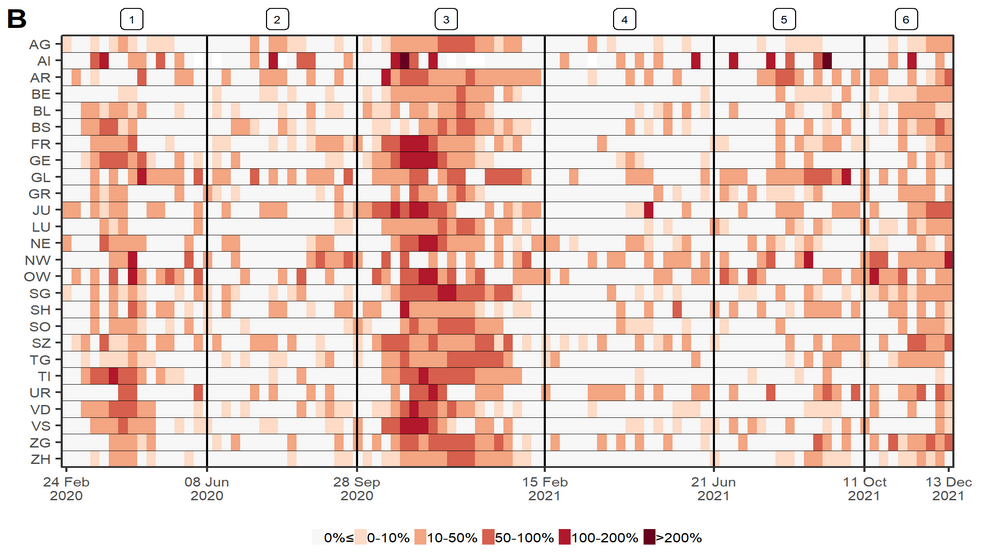
\includegraphics[width=\linewidth ]{excess_fig}
	\caption{Weekly excess mortality in Switzerland in 2020-2021 by canton (epidemic phases 1 to 6 as defined by the BAG).}
\end{figure}
\end{frame}

\begin{frame}
\frametitle{Results: Excess mortality}
\begin{figure}[t]
	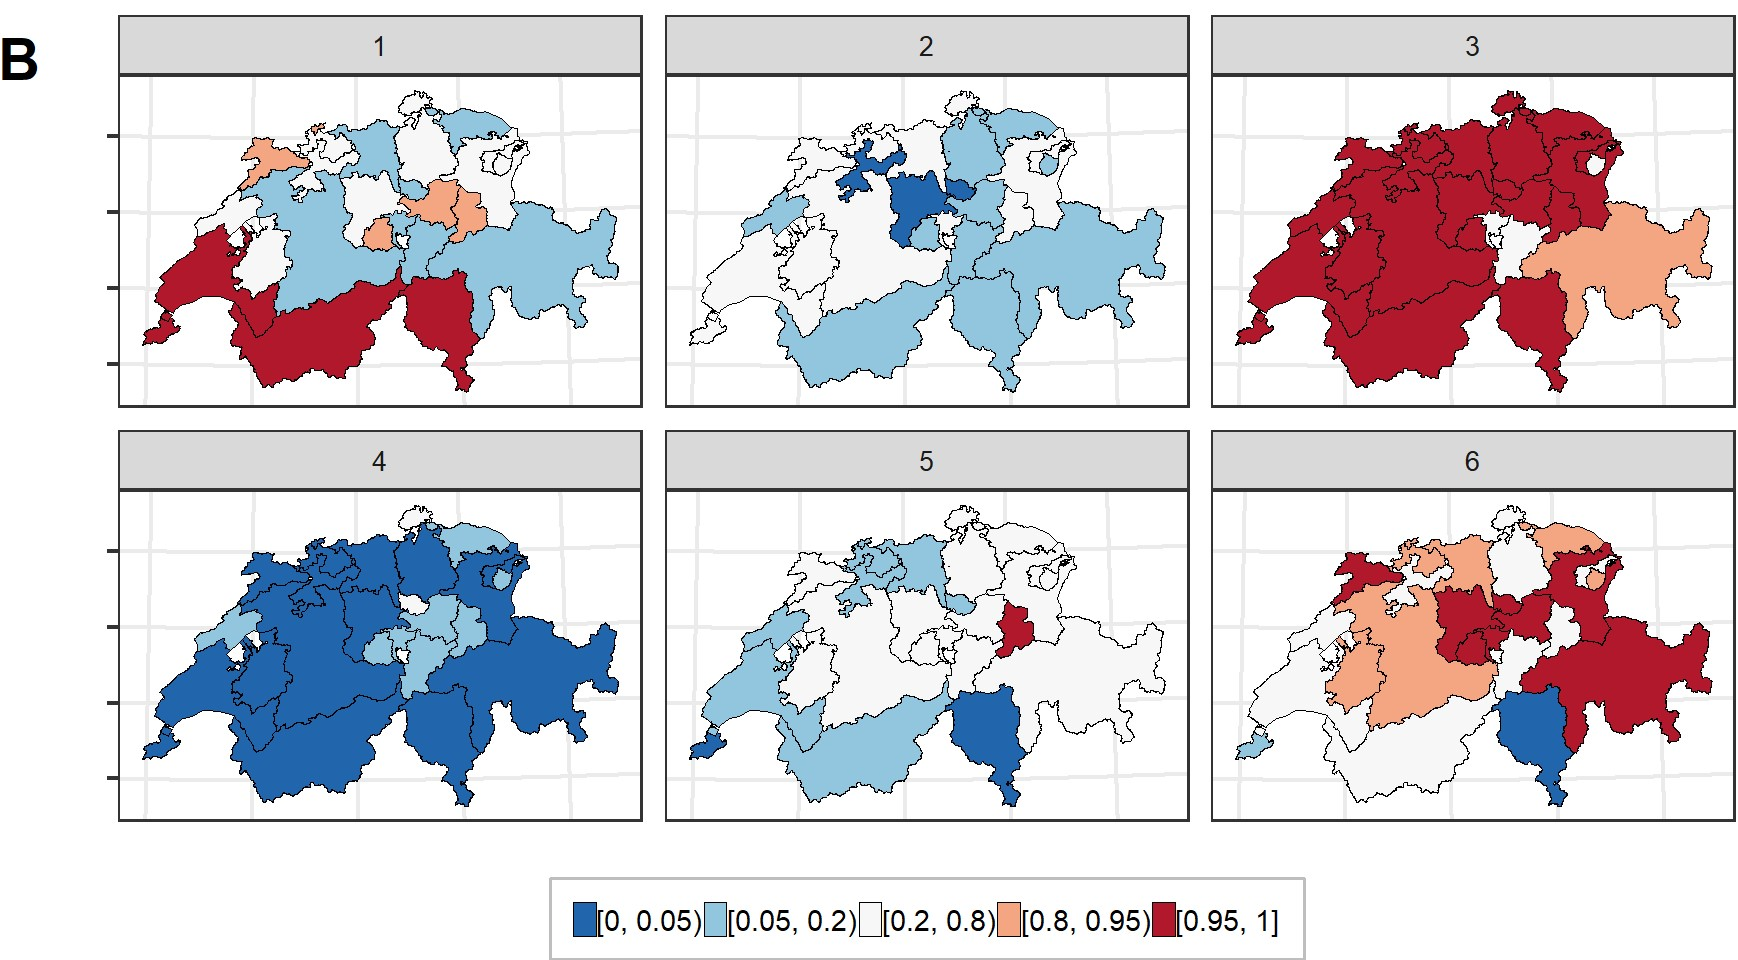
\includegraphics[width=\linewidth ]{spatial_excess}
	\caption{Probability of excess mortality in Switzerland by canton for each epidemic phase.}
\end{figure}
\end{frame}

\begin{frame}
\frametitle{Step 2: excess mortality vs. SARS-CoV-2 deaths}
\alert{Visual comparison} between:
\begin{itemize}
	\item estimated excess all-cause deaths
	\item laboratory-confirmed SARS-CoV-2-related deaths
\end{itemize}
\begin{figure}[t]
		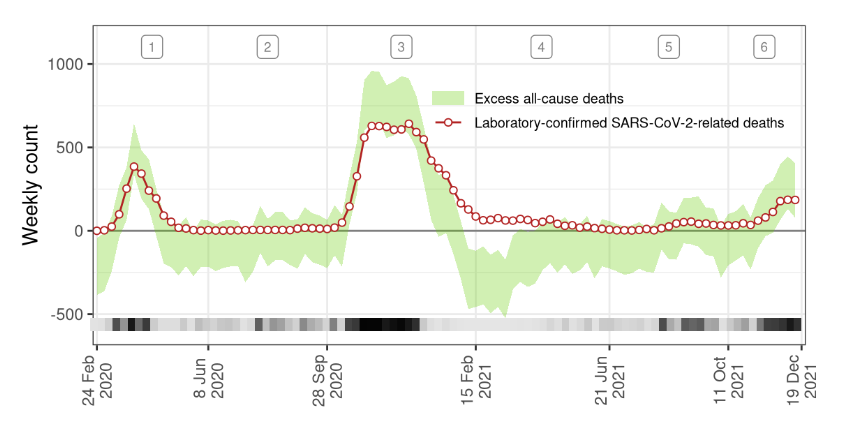
\includegraphics[width=0.9\linewidth ]{visual_comp_fig.png}
	\caption{Excess all-cause deaths and laboratory-confirmed SARS-CoV-2-related deaths in Switzerland in 2020-2021 over time.}
	
\end{figure}
\end{frame}


\begin{frame}
\frametitle{Step 2: excess mortality vs. SARS-CoV-2 deaths}
\alert{Statistical approach} using modified Poisson regression (no intercept):
$$\text{O}_{t} \sim \text{Poisson}\left( \beta_1\text{L}_{t} + \beta_2\text{E}_{t} \right)$$
where:
\begin{itemize}
\item $\text{O}_{t}$ is the observed number of all-cause deaths on week $t$
\item $\text{L}_{t}$ is the number of laboratory-confirmed SARS-CoV-2 deaths
\item $\text{E}_{t}$ is the expected number of all-cause deaths given historical trends
\end{itemize}
\end{frame}


\begin{frame}
\frametitle{Step 2: excess mortality vs. SARS-CoV-2 deaths}
$$\text{O}_{t} \sim \text{Poisson}\left( \alert{\beta_1\text{L}_{t}} + \beta_2\text{E}_{t} \right)$$
\bigskip

\underline{\smash{Interpretation}}: $\beta_1$ is the additional number of observed deaths \alert{for each unit increase in laboratory-confirmed deaths}, controlling for expected deaths:
	\begin{itemize}
		\item if $\beta_1=1$ $\rightarrow$ perfect ascertainment of SARS-CoV-2 deaths
		\item if $\beta_1>1$ $\rightarrow$ more deaths attributable to SARS-CoV-2 than laboratory-confirmed deaths
	\end{itemize}
\bigskip

\alert{$\Rightarrow$} $\beta_1$ measures the \alert{direct effect} of the pandemic on mortality 
\bigskip

\alert{$\Rightarrow$} $\beta_1 \times \text{L}_{t}$ is the total number of deaths directly attributable to SARS-CoV-2 infections
\bigskip

\alert{$\Rightarrow$} $1/\beta_1$ corresponds to the ascertainment of SARS-CoV-2-related deaths

\end{frame}

\begin{frame}
	\frametitle{Step 2: excess mortality vs. SARS-CoV-2 deaths}
	$$\text{O}_{t} \sim \text{Poisson}\left( \beta_1\text{L}_{t} + \alert{\beta_2\text{E}_{t}} \right)$$
	\bigskip
	
	\underline{\smash{Interpretation}}: $\beta_2$ is the additional number of observed deaths \alert{for each unit increase in the expected number of all-cause deaths}, controlling for SARS-CoV-2 deaths:
	\begin{itemize}
		\item if $\beta_2=1$ $\rightarrow$ as many ``all-cause-except-SARS-CoV-2'' deaths than expected
		\item if $\beta_2<1$ $\rightarrow$ fewer ``all-cause-except-SARS-CoV-2'' deaths than expected
	\end{itemize}
	\bigskip
	
	\alert{$\Rightarrow$} $\beta_2$ measures the \alert{indirect effect} of the pandemic on mortality
	
\end{frame}
%
%\begin{frame}
%\frametitle{Step 2: compare excess mortality with COVID-19 related deaths}
%$$\text{O}_{t} \sim \text{Poisson}\left( \beta_1\text{L}_{t} + \beta_2\text{E}_{t} \right),$$
%
%
%\begin{itemize}
%	\item $\beta_2$: number of all-cause deaths for each unit increase in the expected number of all-cause deaths.
%	\begin{itemize}
%		\item \textbf{indirect effect} of pandemic: remaining deaths not attributable to SARS-CoV-2 infections.
%		\item $\beta_2=1$: net effect of pandemic-related changes (behaviour, health system) on death is 0.
%		\item $\beta_2<1$: fewer deaths than expected after removing direct SARS-CoV-2 deaths (i.e. due to protective control measures).
%	\end{itemize}
%\end{itemize} 
%\end{frame}
%
%
%\begin{frame}
%\frametitle{Result: direct and indirect effect on deaths}
%\begin{figure}[t]
%	\includegraphics[width=\linewidth ]{fig4ab.PNG}
%	\caption{$\beta_1$ and $\beta_2$ according to epidemic phases, age groups and cantons.}
%	
%\end{figure}
%\end{frame}

\begin{frame}
\frametitle{Result: direct effect}
        Overall $\beta_1$ is estimated to \alert{1.45 (95\% CrI: 1.33 to 1.57)}:
        
        \begin{itemize}
        	\item 33\% to 57\% more deaths directly attributable to SARS-CoV-2 than confirmed over the whole period
        
            \item 64\% to 75\% ($1/\beta_1$) of deaths directly attributable to SARS-CoV-2 have been ascertained
            
      \end{itemize}
  \bigskip
  
  Estimates by epidemic phase, age group and canton:
%  \begin{itemize}
%        
%        	\item higher in phases 5-6: lower ascertainment?
%        	
%        	\item higher for 80+: lower ascertainment in nursing homes?
%             
%         \item relatively homogeneous in space
% \end{itemize}
    \begin{figure}[t]
	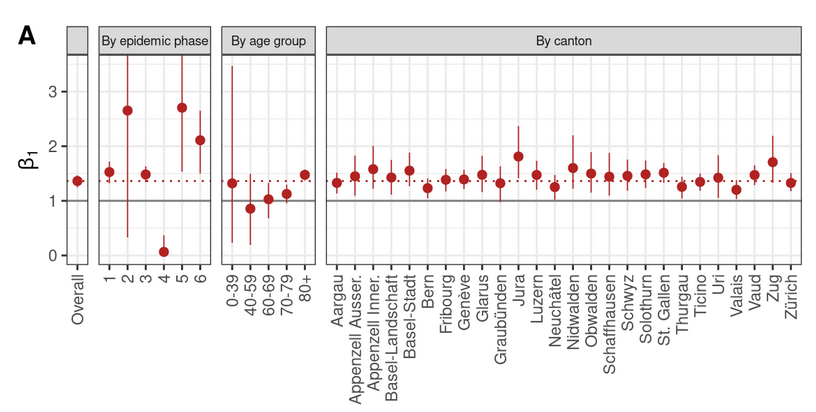
\includegraphics[width=.85\linewidth ]{beta1_fig}
%	\caption{Estimates of $\beta_1$ overall, by epidemic phase, by age group and by canton.}
\end{figure}
\end{frame}

\begin{frame}
	\frametitle{Result:  direct effect}
	
	\begin{figure}[t]
		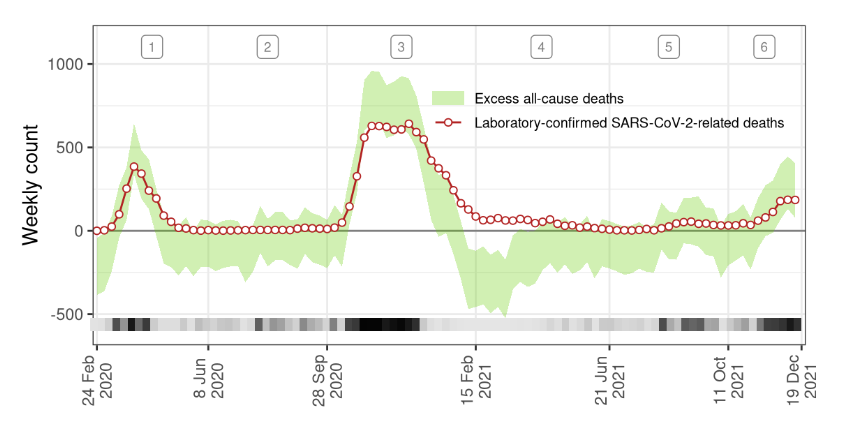
\includegraphics[width=0.9\linewidth ]{visual_comp_fig}
		\caption{Excess all-cause deaths and laboratory-confirmed SARS-CoV-2-related deaths in Switzerland in 2020-2021 over time.}
		
	\end{figure}
\end{frame}

\begin{frame}
\frametitle{Result:  indirect effect}
        Overall $\beta_2$ is estimated to \alert{0.91 (95\% CrI: 0.86 to 0.96)}:
         \begin{itemize}
        	\item 4\% to 14\% fewer ``all-cause-except-SARS-CoV-2'' deaths than expected 
        	\item multiple indistinguishable causes: mortality \alert{displacement}, \alert{protective effect} of control measures (traffic, influenza...)
        \end{itemize}
        \bigskip
        Estimates by epidemic phase, age group and canton:
        
%  \alert{$\bullet$} 9\% fewer deaths that are not attributable to SARS-CoV-2:\vspace*{-0.4\baselineskip}
% %9\% fewer deaths than expected after adjusting for SARS-CoV-2 mortality:
%\begin{itemize}
%\item overestimation of expected mortality -> underestimation of $\beta_2$,\vspace*{-0.2\baselineskip}
%\item mortality displacement,\vspace*{-0.2\baselineskip}
%\item indirect effect of pandemic (control measures). \vspace*{-0.4\baselineskip}
%\end{itemize}
%%\alert{$\bullet$}  $\beta_2$ lower for phases 4:  death displacement.\\
%\alert{$\bullet$} $\beta_2$ lower for 80+:  stronger effect of control measures on elderly.\\%flu
%\alert{$\bullet$} $\beta_2$ homogeneous over the cantons.\\
\begin{figure}[t]
	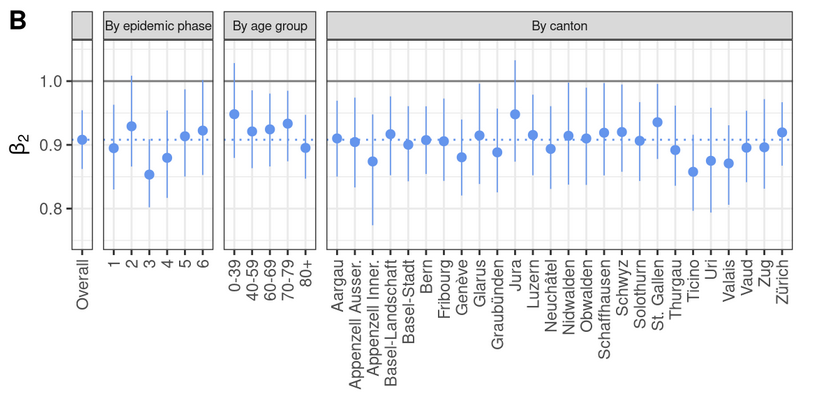
\includegraphics[width=.85\linewidth ]{beta2_fig}
%	\caption{$\beta_2$ according to epidemic phases, age groups and cantons.}
\end{figure}
\end{frame}


\begin{frame}
\frametitle{Result:  indirect effect}

	\begin{figure}[t]
		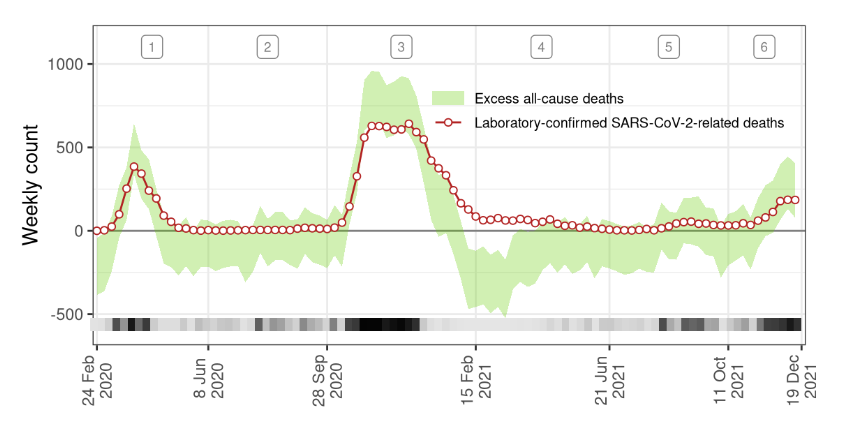
\includegraphics[width=\linewidth ]{visual_comp_fig.png}
		\caption{Excess all-cause deaths and laboratory-confirmed SARS-CoV-2-related deaths in Switzerland in 2020-2021 over time.}
		
	\end{figure}
\end{frame}



\begin{frame}
\frametitle{Conclusions}
\alert{New insights}:
\begin{itemize}
	\item new approach to distinguish between deaths attributable to SARS-CoV-2 infections and deaths from other causes
	\item quantification of the \alert{ascertainment} of SARS-CoV-2-related deaths
	\item quantification of the \alert{indirect effects} of the SARS-CoV-2 pandemic on mortality (displacement + protective effects of control measures)
	\item consistent effects by age group (80+)
	\item homogeneous across cantons
\end{itemize} \bigskip


\alert{Limitations}:
\begin{itemize}
\item the estimate $\beta_2$ relies on the accuracy of the estimated expected mortality (underestimation?)
\item simple linear model: interpretation results with caution
\end{itemize}

\end{frame}


\end{document}